% © Copyright Brayden Price 2024

% This file is part of Brayden's AP Calculus AB Notes.

% Brayden's AP Calculus AB Notes is free software: you can redistribute it and/or modify it under the terms of the GNU General Public License as published by the Free Software Foundation, either version 3 of the License, or (at your option) any later version.

% Brayden's AP Calculus AB Notes is distributed in the hope that it will be useful, but WITHOUT ANY WARRANTY; without even the implied warranty of MERCHANTABILITY or FITNESS FOR A PARTICULAR PURPOSE. See the GNU General Public License for more details.

% You should have received a copy of the GNU General Public License along with Brayden's AP Calculus AB Notes. If not, see <https://www.gnu.org/licenses/>.

%%TO_DO : Questions 4 to 14
\documentclass[12pt,letterpaper, onecolumn]{exam}
\usepackage{amsmath}
\usepackage{amssymb}
\usepackage{nicefrac}
\usepackage{graphicx}
\usepackage{tocbasic}
\usepackage{hyperref}

\usepackage{xcolor}
\hypersetup{
	colorlinks=true,
	linkcolor=blue,
	filecolor=magenta,      
	urlcolor=cyan,
}

\usepackage[lmargin=71pt, tmargin=1.2in]{geometry}  %For centering solution box
\lhead{AP Calculus AB -- APC 4.3 -- 4.4 Assignment\\}
\rhead{Brayden Price\\}
% \chead{\hline} % Un-comment to draw line below header
\thispagestyle{empty}   %For removing header/footer from page 1
\newcommand\at[2]{\left.#1\right|_{#2}}


\DeclareNewTOC[%
type=exercise,%
types=exercises,%
name=Exercise,%
listname={List of Questions},%
tocentrystyle=tocline,%
tocentryindent=0pt,%
tocentrydynnumwidth,%
tocentrypagenumberformat=\entryprefix{page~},%
tocentrypagenumberbox=\mbox
]{exr}
\newcommand*\entryprefix[2]{#1#2}

\qformat{%
	\textbf{Question~\thequestion}%
	\addxcontentsline{exr}{exercise}{Question~\thequestion}%
	\hfill\thepoints%
}

% Command for Line Segment 
\newcommand{\lineSeg}[1]{\overline{\mathrm{#1}}}

\begin{document}
	
	\begingroup  
	\centering
	\LARGE AP Calculus AB\\
	\LARGE AP Classroom: 4.3 -- 4.4\\[0.5em]
	\large \today\\[0.5em]
	\large Brayden Price \\
	All final solutions are \boxed{boxed} \\
	\endgroup
	\rule{\textwidth}{0.4pt}
	
	\listofexercises
	\clearpage
	
	\printanswers
	\renewcommand{\solutiontitle}{\noindent\textbf{Solution:}\enspace}   %Replace "Ans:" with starting keyword in solution box
	
	\begin{questions}
		
		%Q1
		\question
			%BEGIN_FOLD
			\begin{tabular}{l||l|l|l|l}
			 $x$ &  $f(x)$ &  $f^{\prime}(x)$ &  $g(x)$ & $g^{\prime}(x)$ \\ \hline \hline
			 1 &  6    &  4     &  2    & 5     \\
			 2 &  9    &  2     &  3    & 1     \\
			 3 &  10   &  -4    &  4    & 2     \\
			 4 &  -1   &  3     &  6    & 7    
			\end{tabular} \\
			The functions $f$ and $g$ are differentiable for all real numbers, and $g$ is strictly increasing. The table above gives values of the functions and their first derivatives at selected values of $x$. The function $h$ is given by $h(x) = f(g(x)) - 6$. \\
			If $g^{-1}$ is the inverse function of $g$, write an equation for the line tangent to the graph of $y = g^{-1}$ at $x=2$.
		
			\begin{solution}
				Given that $g(1) = 2$, the point of tangency on the graph of $y = g^{-1}$ is the point $(2,1)$. {\footnotesize (since $g^{-1}$ is an inverse of $g$, $g(2)=1$.)} \\
				We now want to find the derivative at the point of tangency: \\ 
				To find $\left[ g^{-1} \right] ^ {\prime} \left( 2 \right)$, we must use the rule for derivatives of inverses:
				\begin{align*}
					\left[ g^{-1} \right] ^ {\prime} \left( x \right) &= \frac { 1 } { g^{\prime} \left( g^{-1} \left( x \right)  \right) } \\
					\left[ g^{-1} \right] ^ {\prime} \left( 2 \right) &= \frac { 1 } { g^{\prime} \left( g^{-1} \left( 2 \right)  \right) } \\
																	  &= \frac { 1 } { g^{\prime} \left( 1 \right) } \\
																	  &= \frac { 1 } { 5 }
				\end{align*}
				Now, we just need to use the point $(2,1)$ and the derivative at that point to write the tangent line: \\
				$$ \boxed{y-1 = \nicefrac{1}{5} \left( x-2 \right)} $$
			\end{solution}
		%END_FOLD
		
		%Q2
		\question A student attempted to confirm that the function $f$ defined by $f(x) = \frac{ x^2 + x - 6}{x^2 -7x + 10}$ is continuous at $x = 2$
			%BEGIN_FOLD
		In which step, if any, does an error first appear?
			\begin{enumerate}
					\item [Step 1:] $$f(x) = \frac {x^2 + x - 6} {x^2 - 7x + 10} = \frac { (x-2) (x+3) } { (x-2) (x-5) }$$
					\item [Step 2:] $$ \lim_{x \to 2} f(x) = \lim_{x \to 2} \frac {x+3}{x-5} = \frac {2+3}{2-5} = - \frac{5}{3}$$
					\item [Step 3:] $$f(2) = \frac {2+3}{2-5} = - \frac{5}{3}$$
					\item [Step 4:] $$ \lim_{x \to 2} f(x) = f(2) \text{, so } f \text{ is continuous at } x=2.$$
			\end{enumerate}
			\begin{solution}
				During Step 3, we made a little bit of a mistake. While in the limit in Step 2, we can simplify the rational definition of $f(x)$, when finding the actual value (or lack thereof) of $f(2)$, we \textbf{\emph{cannot}} do this. \\
				Even though $f$ is actually undefined at $x=2$ (removable discontinuity / hole), we incorrectly said it was equal to $\frac{-5}{3}$, and therefore incorrectly stated $f$ as continuous at $x=2$. 
			\end{solution}
		%END_FOLD
		
		%Q3
		\question Two particles move along the $x$-axis with velocities given by $v_1(t) = -3t^2 + 8t +5$ and $v_2(t) = \sin t$ for time $t \geq 0$. At what time $t$ do the two particles have equal acceleration?
			\begin{solution}
			
		
				To find acceleration from give velocity equations, we must take the derivative of the velocity functions to find two new acceleration equations
				\begin{align*}
					a_1(t) &= \frac{d}{dx} \left( v_1(t) \right) \\
							&= \frac{d}{dx} \left( -3t^2 + 8t +5 \right) \\
							&= -6t + 8 \\ \\
					a_2(t)	&= \frac{d}{dx} \left( v_2(t) \right) \\
							&= \frac{d}{dx} \left( \sin t \right) \\
							&= \cos t \\
				\end{align*}
				Now, we need to find the time $t$ where $a_1(t)=a_2(t)$
				\begin{align*}
					a_1(t) 	&= a_2(t) \\
					-6t + 8 &= \cos t
				\end{align*}
				Since this is a calculator required question, just use your calculator to find the intersection of the line and the cosine function. (\textbf{Make sure your calculator is in radian mode.})
				$$\boxed{t\approx 1.2866}$$
			\end{solution}
	
		%Q4
		\question 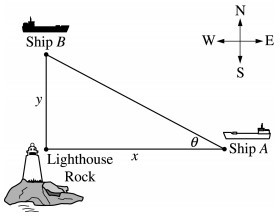
\includegraphics[width=0.7\linewidth]{Question04-001} \\ 
		Ship $A$ is traveling due west toward Lighthouse Rock at a speed of $15$ kilometers per hour (km/hr). Ship $B$ is traveling due north away from Lighthouse rock at a speed of $10$ km/hr. Let $x$ be the distance between Ship $A$ and Lighthouse Rock at time $t$, and let $y$ be the distance between Ship $B$ and Lighthouse Rock at time $t$, as shown in the figure above.
			\begin{solution}
				\vfill
				Equation (Pythagorean Theorem) of situation: $c^2=y^2+x^2$
				Find: $\frac{dc}{dt}$ \\
				When: $x=4$ km and $y=3$ km
				Other Rates: $\frac{dx}{dt} = -15 \frac{\text{km}}{\text{hr}}$ and $\frac{dy}{dt} = 10 \frac{\text{km}}{\text{hr}}$ \\
				$c$ is the hypotenuse / distance between Ship $B$ and Ship $A$. \\
				Using Pythagorean Theorem: $ c = \sqrt{4^2 + 3^2} = 5 $ \\ \\ 
				Find derivative of equation:
				$$\frac{dc}{dt} \cdot 2c = \frac{dy}{dt} \cdot 2y + \frac{dx}{dt} \cdot 2x$$
				Solve for $\frac{dc}{dt}$:
				$$\frac{dc}{dt}  = \frac{\frac{dy}{dt} \cdot 2y + \frac{dx}{dt} \cdot 2x}{2c}$$
				Plug in knowns and solve:
				$$\frac{dc}{dt}  = \frac{10 \cdot 2(3) - 15 \cdot 2(4)}{2(5)} = \frac{60-120}{10} = - \frac{60}{10} = \boxed{-6 \frac{\text{km}}{\text{hr}}}$$
			\end{solution}
		%Q5
		\question Consider the curve give by $y^2=2+xy$ \\
		Let $x$ and $y$ be functions of time $t$ that are related by the equation $y^2 = 2 + xy$. At time $t=5$, the value of $y$ is $3$ and $dy/dt = 6$. Find the value of $dx/dt$ at time $t=5$.
		\begin{solution}
			Find x at $y=3$ (will be needed later):
			\begin{align*}
				(3)^2 &= 2 + 3x \\
				9 - 2 &= 3x \\
				\frac{7}{3} &= x
			\end{align*}
			Take derivative of given curve and then solve for $dx/dt$:
			\begin{align*}
				2y \cdot \frac{dy}{dt} &= x \cdot \frac{dy}{dt} + y \cdot \frac{dx}{dt} \\
				\frac{ 2y \cdot \frac{dy}{dt} - x \cdot \frac{dy}{dt} } { y } &= \frac{dx}{dt}
			\end{align*}
			Plug in knowns and simplify:
			$$\frac{ 2(3) \cdot 6 - \frac{7}{3} \cdot 6 } { 3 } = \frac{36-14}{3} = \boxed{\frac{22}{3} = \frac{dx}{dt}}$$
		\end{solution}
		%Q6
		\question The radius $r$ of a sphere is increasing at a constant rate of $0.04$ centimeters per second. (Note: The volume $V$ of a sphere with radius $r$ is $V= \nicefrac{4}{3} \pi r^3$.) \\
		At the time when the radius, $r$, of the sphere is 10 centimeters, what is the rate of increase of its volume, $dV/dt$?
		
		\begin{solution}
			Differentiate given equation with respect to $t$ (time):
			$$\frac{dV}{dt} = \frac{4}{3} \pi (3r^2) \left( \frac{dr}{dt}\right) $$
			Plug in knowns and simplify:
			$$\frac{4}{3} \pi (3(10)^2) (0.04) = \frac{4}{3} \pi (12) = \boxed{16\pi = \frac{dV}{dt}}$$
		\end{solution}
		%Q7
		\question 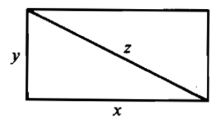
\includegraphics[width=0.35\linewidth]{Question07-001} \\
		The sides of the rectangle above increase in such a way that $\frac{dz}{dt} = 1$ and $\frac{dx}{dt} = 3 \frac{dy}{dt}$. At the instant when $x = 4$ and $y = 3$, what is the value of $\frac{dx}{dt}$?
		
		\begin{solution}
			Write $\frac{dy}{dt}$ in terms of $\frac{dx}{dt}$ (will be needed later):
			$$\frac{1}{3} \cdot \frac{dx}{dt} = \frac{dy}{dt}$$
			Find z using Pythagorean Theorem (will be needed later):
			$$z = \sqrt{4^2+3^2} = 5$$
			Write derivative of Formula for side lengths of triangle (Pythagorean Theorem):
			$$2z\frac{dz}{dt}=2x\frac{dx}{dt} + 2y\frac{dy}{dt}$$
			Solve for $\frac{dx}{dt}$:
			$$\frac{2z\frac{dz}{dt} - 2y\frac{dy}{dt}} {2x} = \frac{dx}{dt}$$
			Plug in knowns and simplify:
			$$\frac{2(5)(1) - 2(3)(\frac{1}{3} \cdot \frac{dx}{dt})} {2(4)} = \frac{10 - 6\left( \frac{1}{3} \cdot \frac{dx}{dt}\right) } {8} =  \frac{10 - 2\frac{dx}{dt}}{8} = \frac{dx}{dt}$$ \\
			$$\frac{dx}{dt} + \frac{2}{8} \left( \frac{dx}{dt}\right)  = \frac{10}{8}$$
			$$\frac{10}{8} \left( \frac{dx}{dt}\right)  = \frac{10}{8}$$
			$$\boxed{\frac{dx}{dt} = 1}$$
		\end{solution}
		
		%Q8
		\question 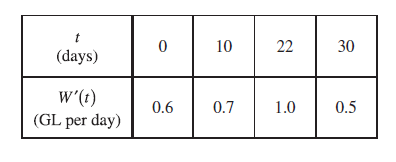
\includegraphics[width=0.5\linewidth]{Question08-001}\\
		The twice-differentiable function W models the volume of water in a reservoir at time $t$, where $W(t)$ is measured in (GL) and $t$ is measured in days. The table above gives values of $W^{\prime}(t)$ sampled at various times during the time interval $0 \leq t \leq 30$ days. At time $t = 30$, the reservoir contains 125 gigaliters of water. \\ \\
		The equation $A = 0.3W^{\nicefrac{2}{3}}$ gives the relationship between the area $A$, in square kilometers, of the surface of the reservoir, and the volume of the water $W(t)$, in gigaliters, in the reservoir. Find the instantaneous rate of change of $A$, in square kilometer per day, with respect to $t$ when $t$ = 30 days.
		\begin{solution}
			We are attempting to find $A^{\prime}(t)$ when $t=30$ days. \\
			Knowns: $W^\prime(30) = 0.5$, $W(30)=125$ and $A=7.5$
			Differentiate given equation for $A$:
			$$A^{\prime} = 0.4(\nicefrac{2}{3}W^{\nicefrac{1}{3}})(W^{\prime})$$
			Plug in and simplify:
			$$\left( \frac{3}{10}\right) \left( \frac{2}{3 \sqrt[3]{125}}\right) \left( \frac{1}{2}\right)  = \frac{6}{300} = \boxed{0.02 = A^{\prime}}$$
		\end{solution}
		%Q9
		\question 
		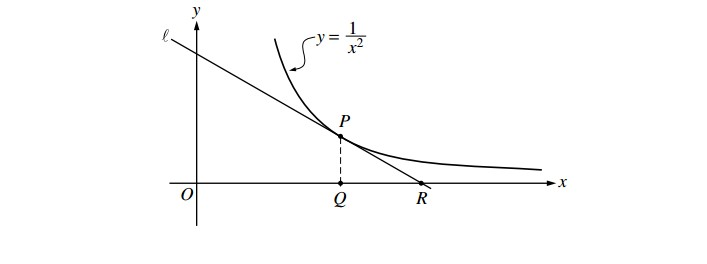
\includegraphics{Question09-001} \\
		In the figure above, line $\ell$ is tangent to the graph of $y = \frac{1}{x^2}$ at point $P$, with coordinates $w,\frac{1}{w^2}$, where $w > 0$. Point $Q$ has coordinates $(w, 0)$. Line $\ell$ crosses the $x$-axis at point $R$, with coordinates $(k, 0)$.
			\begin{parts}
				\part Find the value of $k$ when $w = 3$. 
				\part For all $w > 0$, find $k$ in terms of $w$.
				\part Suppose that $w$ is increasing at the constant rate of 7 units per second. When $w = 5$, what is the rate of change of $k$ with respect to time?
				\part  Suppose that $w$ is increasing at the constant rate of 7 units per second. When $w = 5$, what is the rate of change of the area of $PQR$ with respect to time? Determine whether the area is increasing or decreasing at this instant.
			\end{parts}
			
		\pagebreak
		\begin{solution}
				The slope of the tangent line $\ell$ is $\frac{dy}{dx}\big{|}_{x=w}$ (Since w is the x coordinate of point $P$.) \\
				Derivative of $y$:
				$$\frac{dy}{dx} = \frac{d}{dx} (x ^ {-2}) = -2x^{-3} = \frac{-2}{x^3}$$
				
			\begin{parts}
				\part %a
					In order to find Point $R$, where $y=0$, we should write the equation of line $\ell$ where $x=w$ (the x-coordinate of point $P$) and then plug in $y=0$:
					\begin{align*}
						y-\frac{1}{w^2} &= \left( \frac{dy}{dx}\bigg{|}_{x=w} \right) (k-w) \\
						-\frac{1}{w^2} &= \left( \frac{dy}{dx}\bigg{|}_{x=w} \right) (k-w) 
					\end{align*}
					Now, we need to plug in $w=3$ and solve for x:
					\begin{align*}
						-\frac{1}{3^2}  &= \left( \frac{dy}{dx}\bigg{|}_{x=3} \right) (k-3) \\
						-\frac{1}{9}    &= \left(-\frac{2}{3^3} \right) (k-3) \\
						-\frac{1}{9}    &= \left(-\frac{2}{27} \right) (k-3) \\
						k-3			    &= \frac{-\frac{1}{27}}{-\frac{2}{9}} \\
						k 			    &= \left( -\frac{1}{27} \cdot -\frac{9}{2} \right) + 3 \\
						k 			    &= \boxed {\frac{9}{54} + 3 = \frac{1}{6} + 3 = \frac{19}{6} \approx 3.1667}
					\end{align*}
				\part %b
					\begin{align*}
						-\frac{1}{w^2} &= \left( \frac{dy}{dx}\bigg{|}_{x=w} \right) (k-w) \\
						-\frac{1}{w^2} &= \left( \frac{-2}{w^3} \right) (k-w) \\ 
						k-w &= -\frac{1}{w^2} \div \left( \frac{-2}{w^3} \right) \\
						k &= -\frac{1}{w^2} \left( \frac{w^3}{-2} \right) + w \\
						k &= \frac{w}{2} + w = \boxed{\frac{3w}{2}}
					\end{align*}
				\part %c
					Knowns:
					\begin{gather*}
						\frac{dw}{dt} = 7 \text{units p/ sec} \\
						w=5
					\end{gather*}
					Find $\frac{d}{dt}$ of $k$:
					\begin{align*}
					\frac{dk}{dt} &= \frac{3}{2}\left( \frac{dw}{dt} \right) \\
					\end{align*}
					Plug in Knowns:
					\begin{align*}
					\frac{dk}{dt} &=  \frac{3}{2}\left( 7 \right) \\
					\frac{dk}{dt} &=  \boxed{\frac{21}{2} = 10.5 \text{ units p/ sec}}
					\end{align*}
				\part %d
					\begin{gather*}
						\lineSeg{PQ} = \frac{1}{w^2} - 0 \\
						\lineSeg{QR} = k-w \\ \\
						\frac{dw}{dt} = 7 (\text{given in problem})
						\frac{dk}{dt} = \frac{3}{2}\left( \frac{dw}{dt} \right)
					\end{gather*}
					\begin{align*}
						A &= \frac{1}{2} \left( \lineSeg{QR} \right) \left( \lineSeg{PQ} \right)  \\
						A &= \frac{1}{2} \left( \frac{k-w}{w^2} \right) \\
						A &= \frac{k}{2w^2} - \frac{w}{2w^2} \\
						\frac{dA}{dt} &= \frac{ 2w^2 \left( \frac{d}{dt} \left( k-w \right) \right) }{4w^4} - \frac{\left(   k - w \right) \left( \frac{d}{dt} \left( 2w^2 \right) \right)  }{4w^4} \\
						\frac{dA}{dt} &= \frac{ 2w^2 \left( \frac{dk}{dt} - \frac{dw}{dt} \right) }{4w^4} - \frac{\left(   k - w \right)  \left( 4w \frac{dw}{dt} \right)  }{4w^4} \\
					\end{align*}
					Find $k$  and $\frac{dk}{dt}$ so we can plug them in:
					\begin{align*}
						\frac{dk}{dt} &= \frac{3}{2} (7) = \frac{17}{2} = 8.5\\
						k &= \frac{3w}{2} = \frac{15}{2} = 7.5\\
					\end{align*}
					Plug in $\frac{dw}{dt}, w$ and $\frac{dk}{dt}:$
					\begin{align*}
						\frac{dA}{dt} &= \frac{ (50) \left( 8.5 - 7 \right) }{2500} - \frac{\left( 7.5 - 5 \right)  \left( 20 (7) \right)  }{2500} \\
						\frac{dA}{dt} &= \frac{75 - 350}{2500} = \boxed{-\frac{275}{2500} = -0.11 \text{ units\textsuperscript{2} p/ sec}}
					\end{align*}
			\end{parts}
		\end{solution}
		%Q10
		\question If $f$ is a function that has a removable discontinuity at $x=3$, which of the following could be the graph of $f$?
		\begin{solution}
			This would indicate that the function $f$ is continuous around $x=3$, even if it is not continuous \emph{at} $x=3$.
			The only graph that fulfills this is The one pictured below: \\
			\boxed{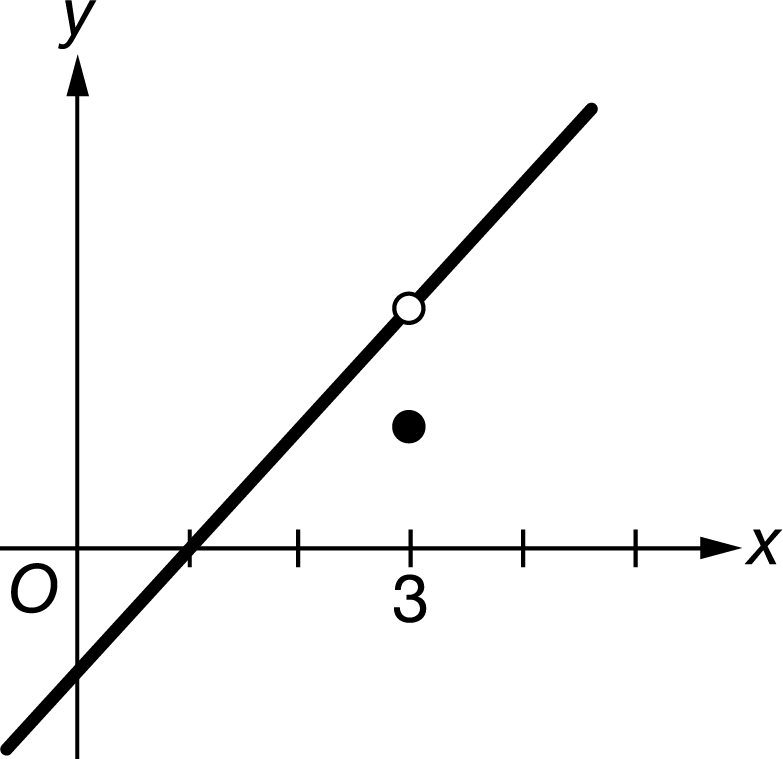
\includegraphics[width=0.4\linewidth]{Question10-001}}
		\end{solution}
		%Q11
		\question
		%Q12
		\question
		%Q13
		\question
		%Q14
		\question
	\end{questions}
\end{document}
